Previo al montaje definitivo del sistema, se llevaron a cabo ensayos de validación sobre protoboard con el fin de verificar el correcto funcionamiento de los motores, el driver L298N y la placa Arduino. Durante esta fase se comprobó la respuesta individual de cada motor ante las señales de control, así como la integridad del sistema de alimentación y del cableado.

En la Figura~\ref{fig:motores} se presentan las conexiones iniciales entre los motores y los módulos L298N. Estas pruebas permitieron determinar la polaridad adecuada de conexión y validar el funcionamiento bidireccional de los motores bajo distintas condiciones de operación.

\begin{figure}[H]
\centering
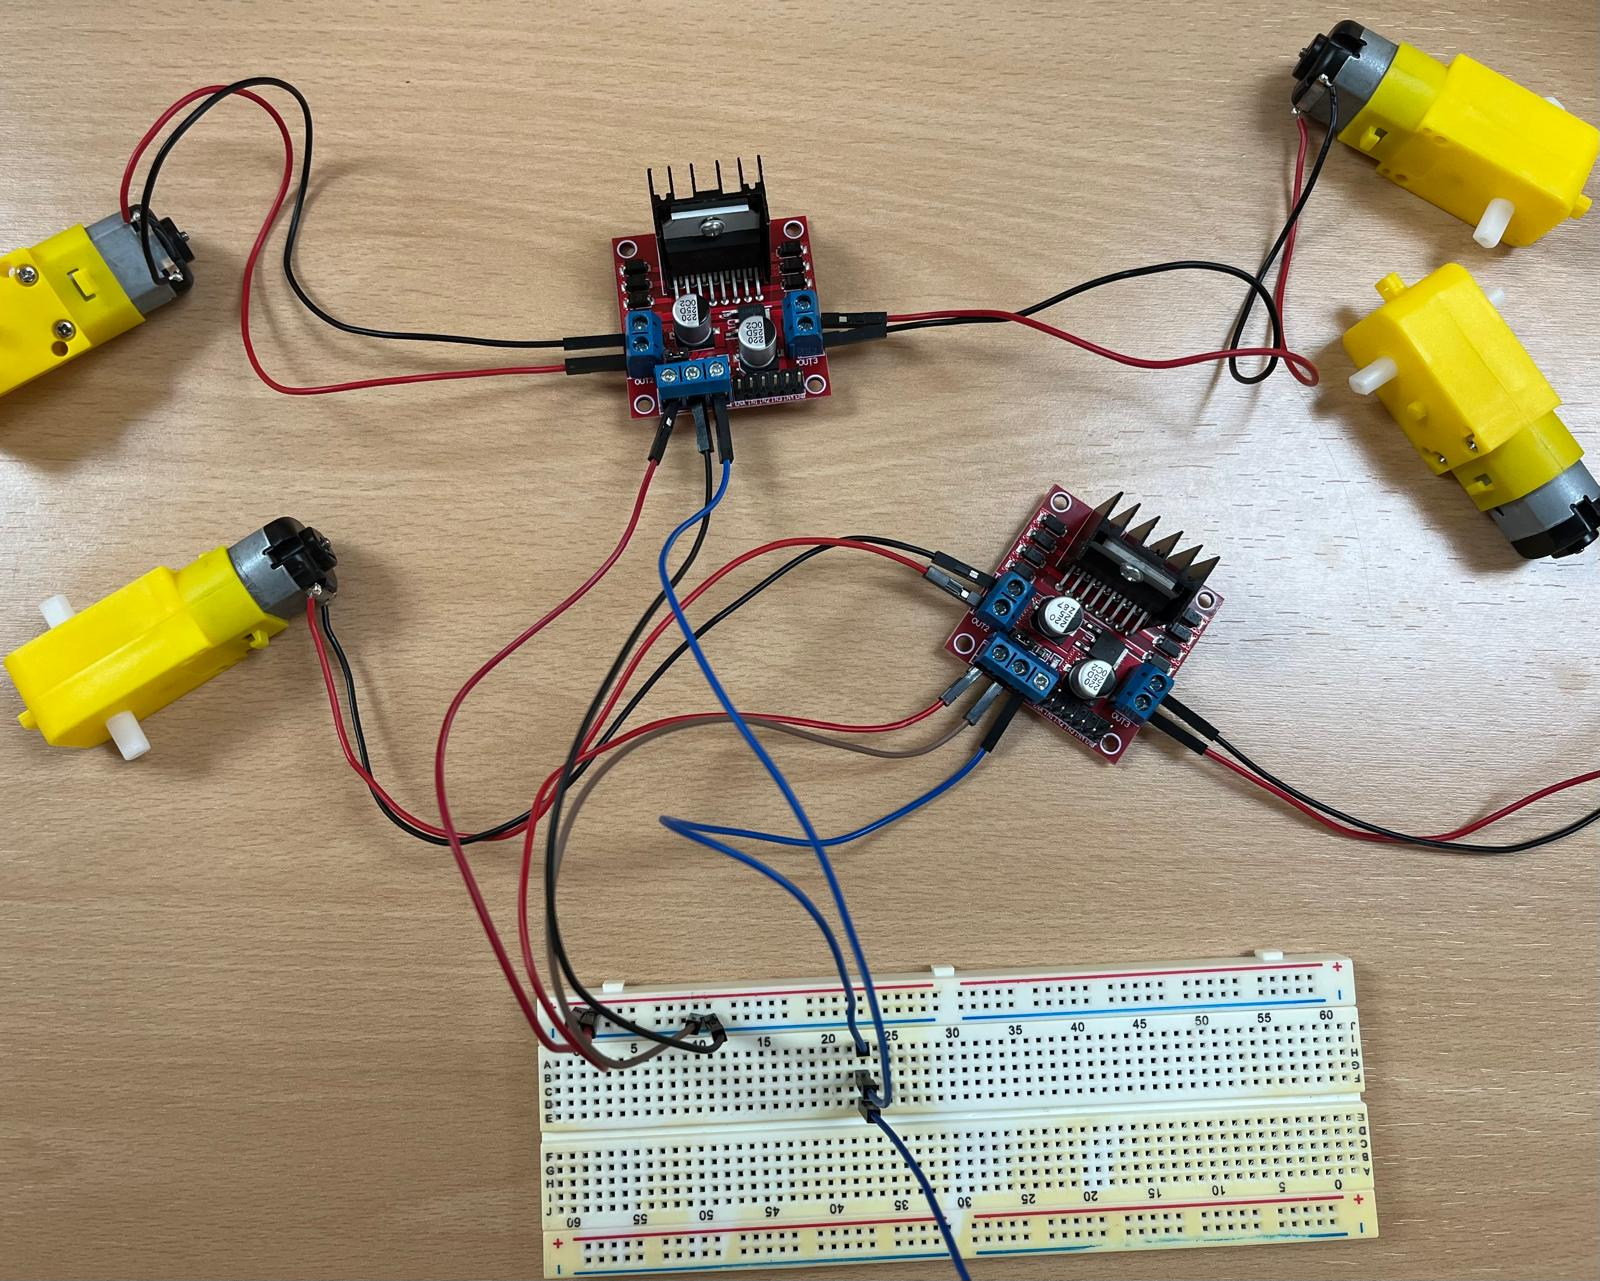
\includegraphics[width=0.5\textwidth]{conexionesCableadoMotores.png}
\caption{Configuración inicial de conexión entre motores y módulos L298N}
\label{fig:motores}
\end{figure}

La Figura~\ref{fig:sistema} muestra la integración del sistema completo, incluyendo la placa Arduino Mega y el protoboard. En esta etapa se verificó la operación simultánea de los motores, evaluando la correcta ejecución del algoritmo de control y la ausencia de interferencias eléctricas o conflictos en las señales.

\begin{figure}[H]
\centering
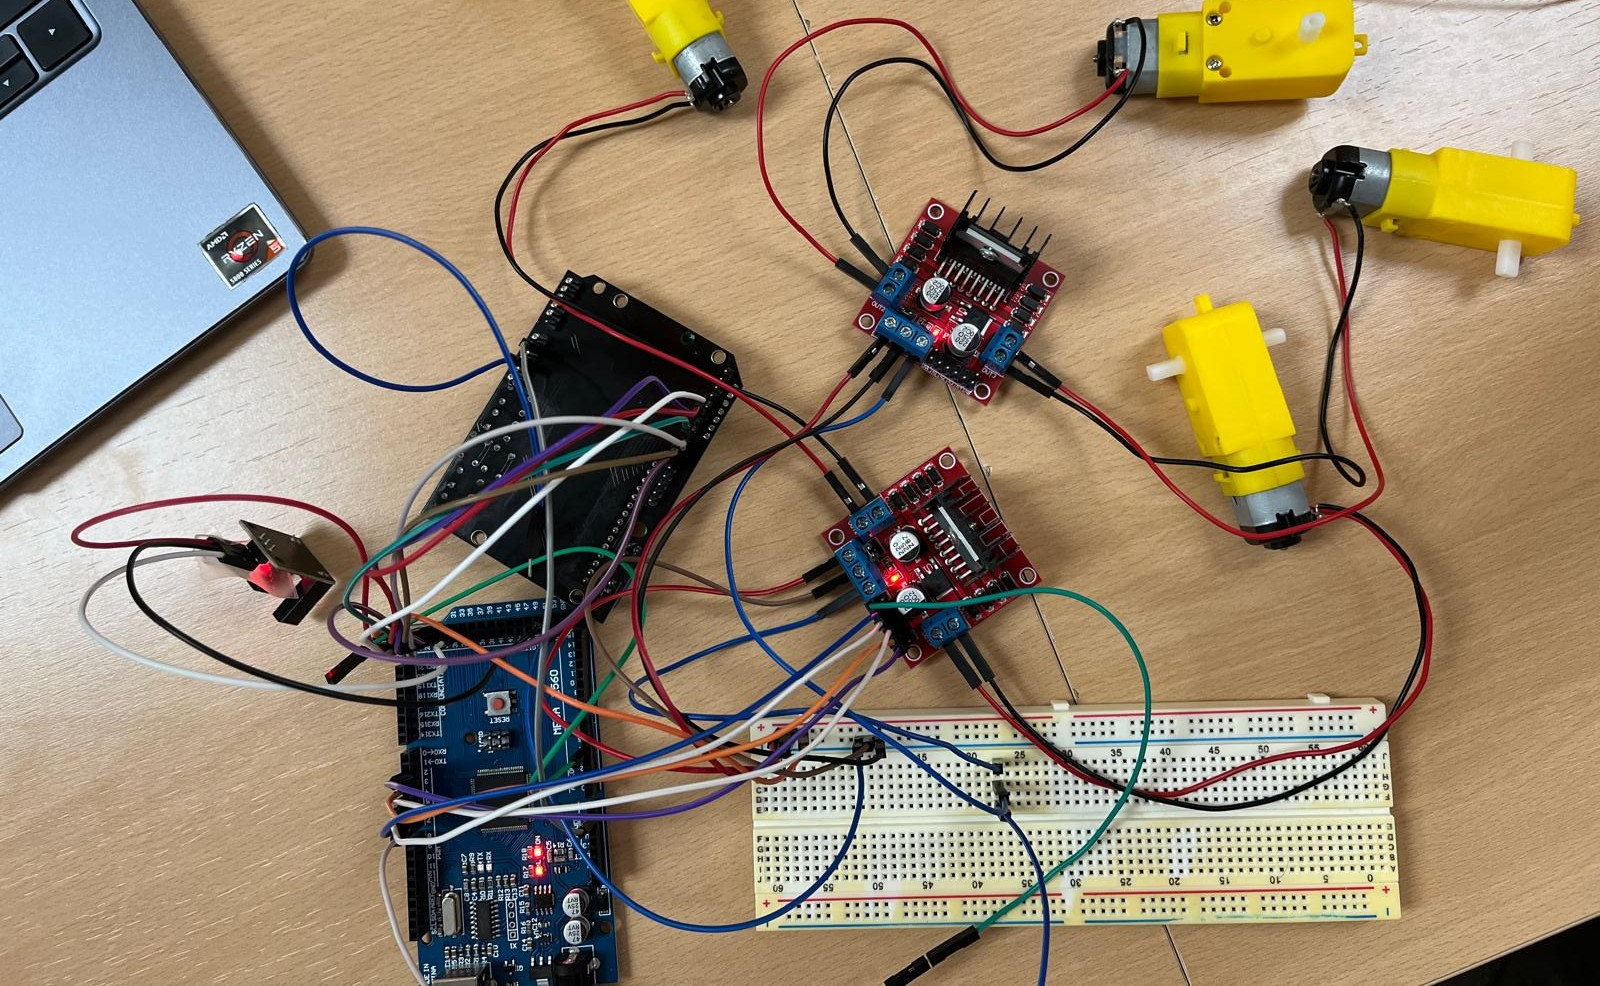
\includegraphics[width=0.65\textwidth]{pruebas_sistema_completo.png}
\caption{Validación funcional del sistema eléctrico con todos los motores en operación}
\label{fig:sistema}
\end{figure}

En la Figura~\ref{fig:pantalla} se observa el sistema en funcionamiento con la interfaz de visualización activa. Esta prueba permitió comprobar la correcta integración de los subsistemas de control y visualización.

\begin{figure}[H]
\centering
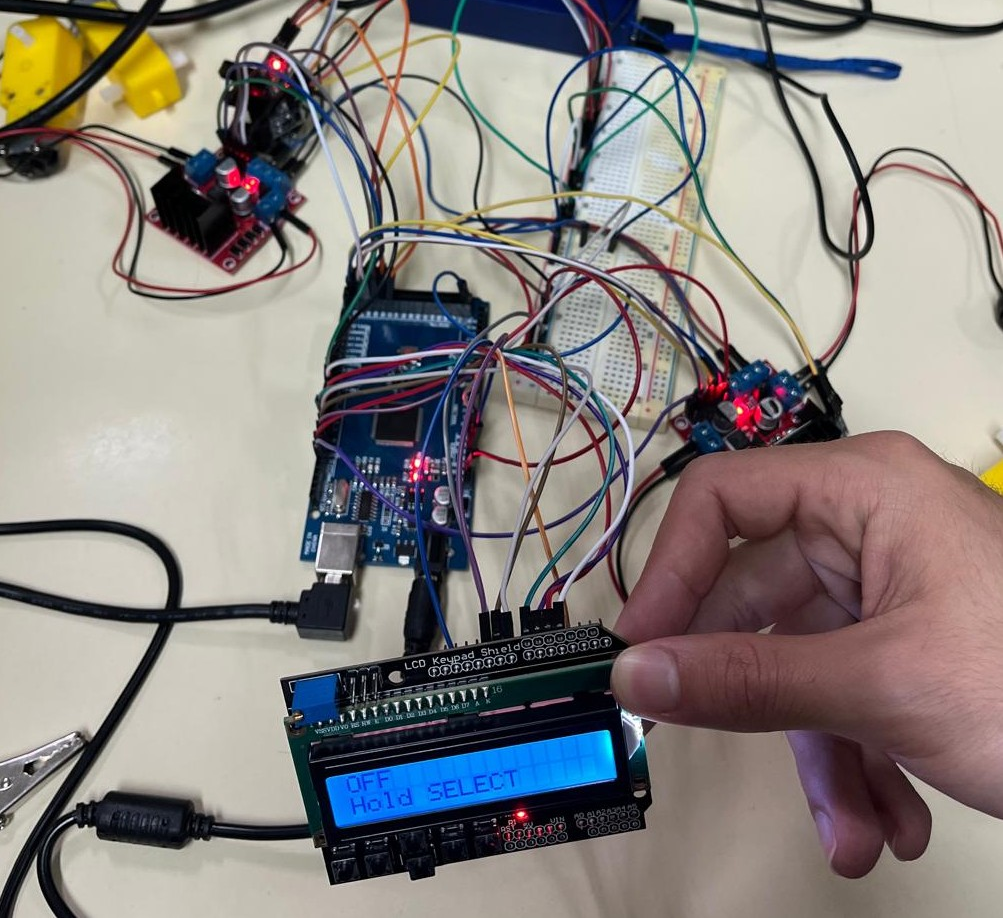
\includegraphics[width=0.6\textwidth]{pantalla encendida.png}
\caption{Sistema en operación con la pantalla activa}
\label{fig:pantalla}
\end{figure}

La Figura~\ref{fig:soldadura} documenta el proceso de soldadura de las conexiones eléctricas, realizado con el objetivo de mejorar la fiabilidad mecánica y eléctrica del sistema frente a conexiones temporales en protoboard.

\begin{figure}[H]
\centering
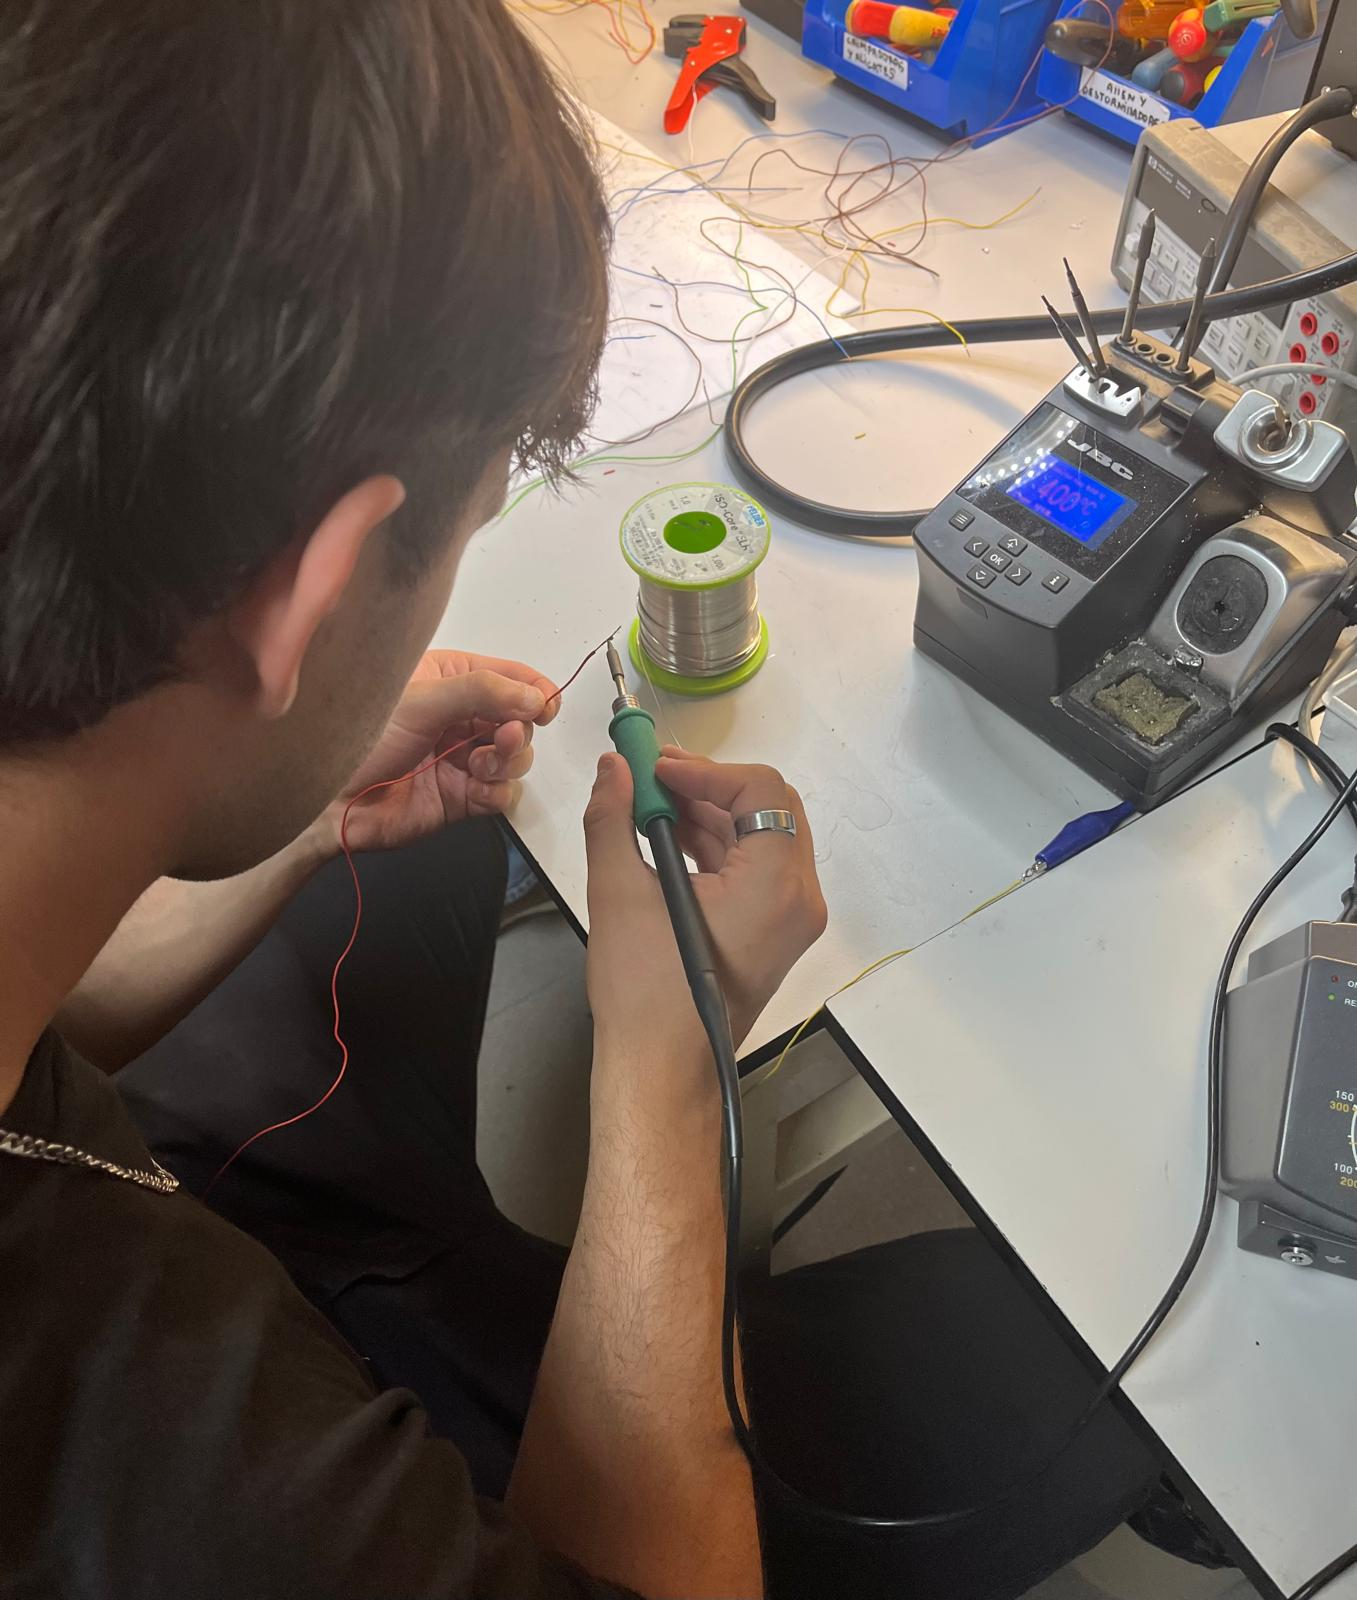
\includegraphics[width=0.6\textwidth]{carre_soldar.png}
\caption{Proceso de soldadura de las conexiones eléctricas}
\label{fig:soldadura}
\end{figure}

Finalmente, en la Figura~\ref{fig:lazy_susan} se presenta el montaje del rodamiento tipo “Lazy Susan”, cuyo diseño se ha basado en la referencia mostrada en el vídeo~\cite{video4}. Este elemento permite el movimiento rotacional del conjunto, garantizando estabilidad y baja fricción durante la operación.

\begin{figure}[H]
\centering
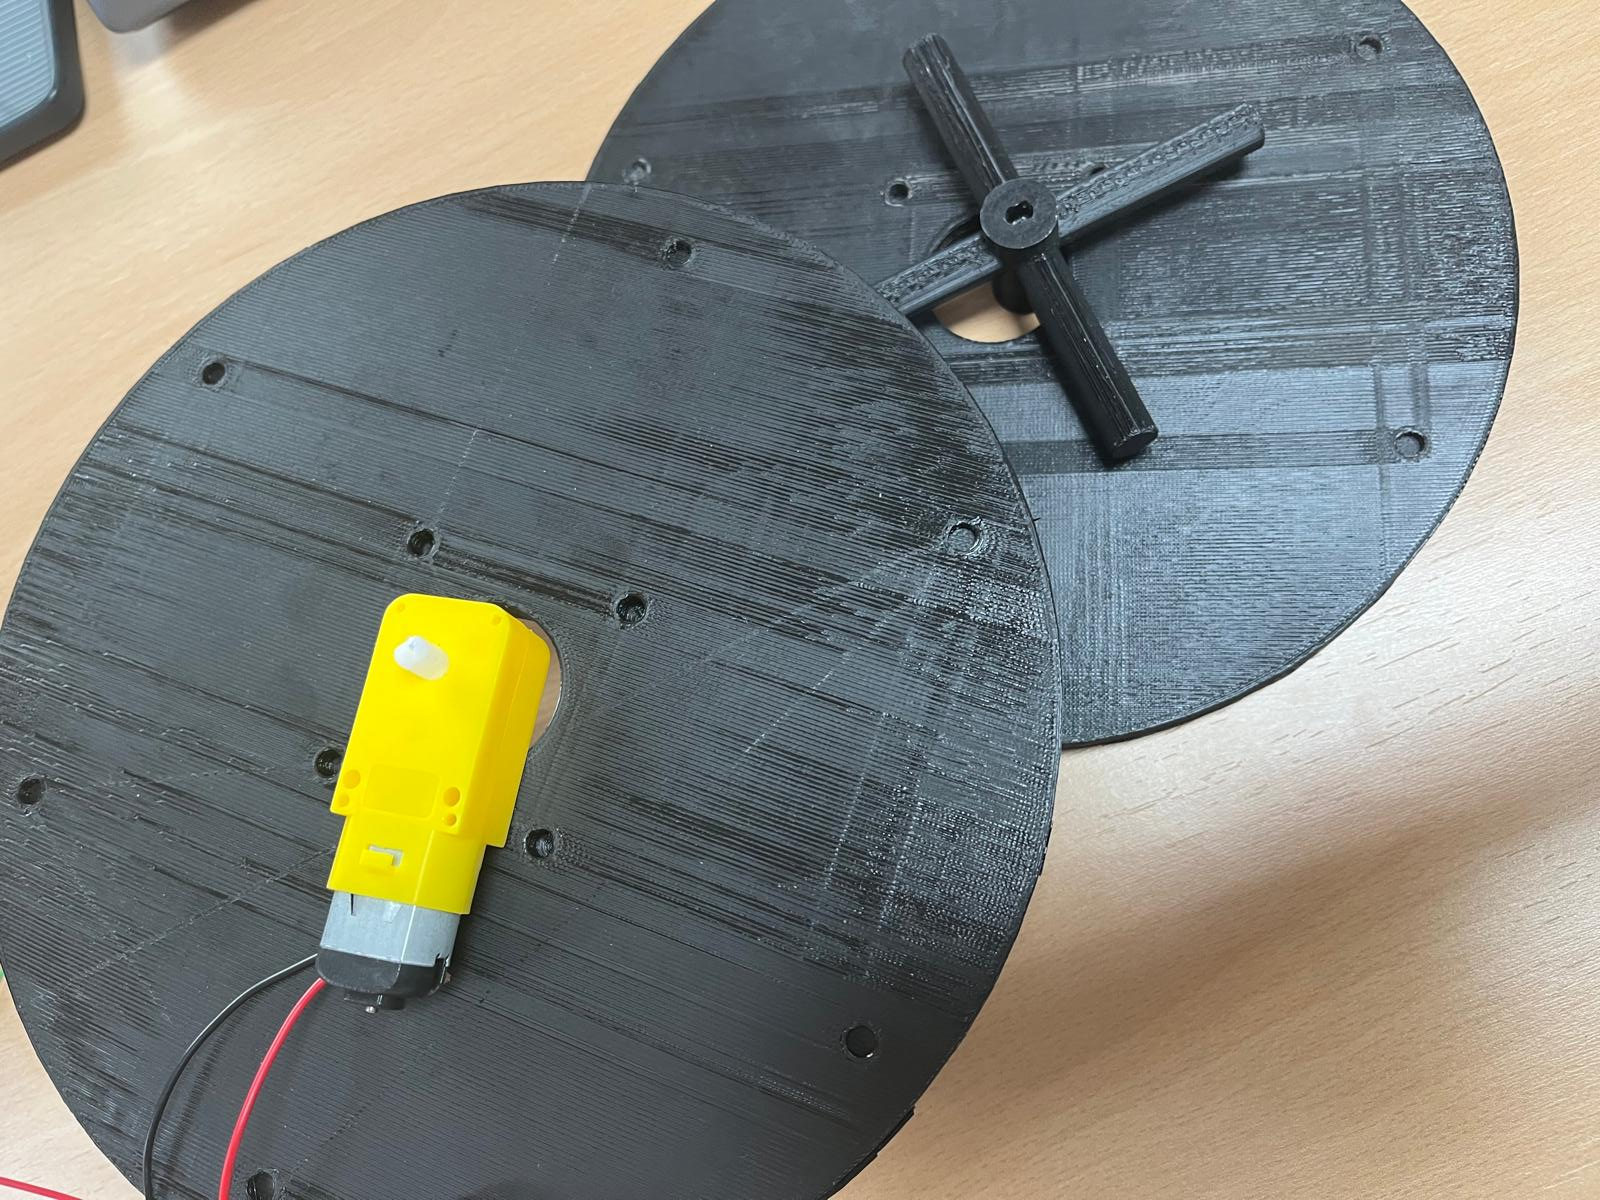
\includegraphics[width=0.65\textwidth]{lazy_susan.png}
\caption{Montaje del rodamiento tipo “Lazy Susan”}
\label{fig:lazy_susan}
\end{figure}

Tras el ensamblaje mecánico, se procedió a la instalación del \textbf{sensor magnético HOME} en la base del rodamiento. Se programó una rutina de inicio en la que el sistema realiza un giro de búsqueda a baja velocidad hasta detectar el imán de referencia. Este proceso permite que la Arduino Mega establezca de forma determinista la posición de 0 grados exactos en cada arranque, garantizando que el reparto posterior sea preciso y no se descalibre con el tiempo.